\chapter{Methodik}
\label{chap:methodik}

Für die Segmentierung der Marsoberfläche wird der Ansatz von Kanezaki \etal \cite{kanezaki_18} aus Unterabschnit~\ref{ssec:kanezaki} abgewandelt. Das Ziel besteht daraus, eine Eingabebilddatei durch neuronale Netze zu segmentieren, allerdings ohne vorhandene Ground Truth.

Zur Modifikation des genannten Algorithmus existieren viele unterschiedliche Möglichkeiten, einzelne Elemente zu ersetzen, welche in den folgenden Abschnitten beschrieben werden.

\section{Initialisierung}
\label{sec:initialisierung}

Die wohl wichtigste Veränderung des ursprünglichen Algorithmus besteht aus der Modifizierung des Initialisierungsalgorithmus.

Der von Kanezaki \etal genutzte SLIC-Algorithmus eignet sich zwar gut für die meisten mehrfarbigen Fotografien, da die Aufnahmen der Marsoberfläche allerdings nur in Graustufen vorhanden sind, würden so hier keine guten Ergebnisse produziert werden.

\begin{figure}[h!]
	\centering
	\begin{subfigure}[t]{0.32\textwidth}
		\centering
		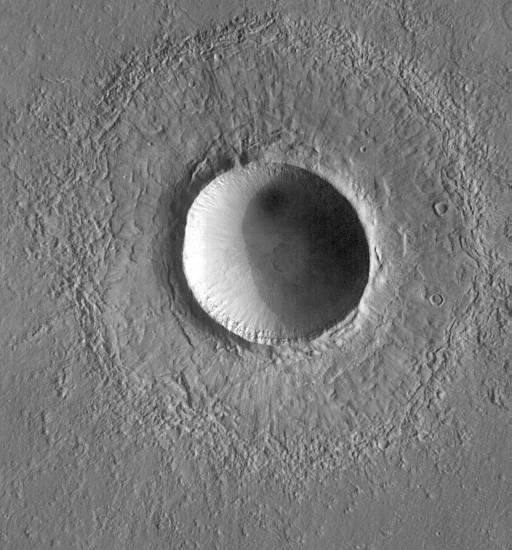
\includegraphics[width=\textwidth,keepaspectratio]{images/Gre13_01.jpg}
		\captionsetup{format=plain,width=0.85\textwidth}
		\caption{Eingabebild, aus \cite[Kap.~7]{greeley_13}}
		\label{fig:slic_vs_tsugf_in}
	\end{subfigure}
	\hfill
	\begin{subfigure}[t]{0.32\textwidth}
		\centering
		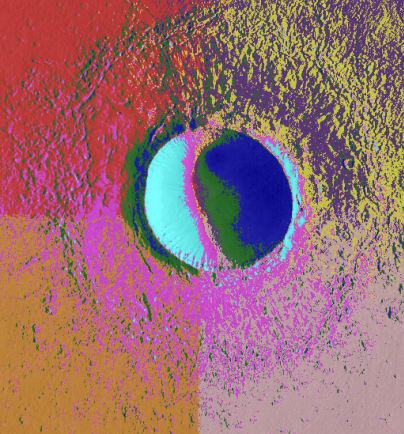
\includegraphics[width=\textwidth,keepaspectratio]{images/gen/GEN_slic_vs_tsugf_01.png}
		\captionsetup{format=plain,width=0.85\textwidth}
		\caption{Ergebnis des SLIC-Algorithmus angewandt auf die Eingabedatei}
		\label{fig:slic_vs_tsugf_slic}
	\end{subfigure}
	\hfill
	\begin{subfigure}[t]{0.32\textwidth}
		\centering
		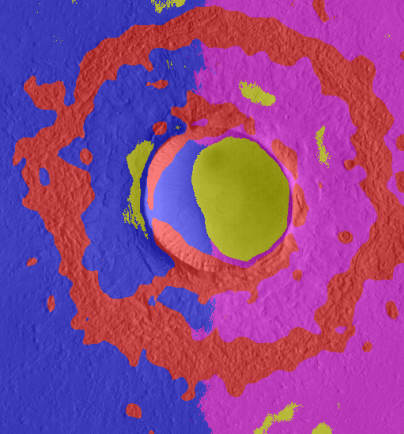
\includegraphics[width=\textwidth,keepaspectratio]{images/gen/GEN_slic_vs_tsugf_02.png}
		\captionsetup{format=plain,width=0.85\textwidth}
		\caption{Ergebnis des texturbasierten Clusterings der Eingabedatei}
		\label{fig:slic_vs_tsugf_tsugf}
	\end{subfigure}
	\caption{Clustering eines Graustufenbildes}
\end{figure}

So ergibt ein Clustering des Kraters aus Unterabschnitt~\ref{ssec:mars_surface} durch den SLIC-Algorithmus \cite{achanta_10} das in \figurename~\ref{fig:slic_vs_tsugf_slic} sichtbare Ergebnis.\footnote{SLIC-Implementierung: \texttt{scikit-image}\\Parameter: \texttt{compactness=5, n\_segments=10, enforce\_connectivity=False}} Dort ist erkennbar, dass der Krater in jeweilige Licht- und Schattenregionen (bedingt durch den Lichteinfall im flachen Winkel) unterteilt wird. Außerdem wird die raue Struktur ringförmig um den Krater herum schlecht erfasst: An dieser Stelle wird jeder Hügel separat als einerseits helle, andererseits dunkle Stelle markiert. Das Phänomen, dass ein Krater so durch eine starke Differenz an Licht- und Schattenregionen äußert wird sich im Großen und Ganzen zwar in Abschnitt~\ref{sec:craterdetection} zu nutze gemacht, ist hier allerdings ungewollt.

Wenn nun der in Unterabschnitt~\ref{ssec:kanezaki} beschriebene Ansatz verfolgt wird, wird das neuronale Netz daraufhin trainiert, eine Aufnahme anhand ihrer Helligkeitsinformationen hin zu trainieren. Da dies nicht gewollt ist, wird statt einem farb-/helligkeitsbasierten Clusteringalgorithmus wie SLIC ein texturbasiertes Clustering genutzt.

Statt des SLIC-Clusterings wird nun die in Unterabschnitt~\ref{ssec:tsugf} vorgestellte Methode des texturbasierten Clusterings genutzt. Das Ergebnis eines Clusterings durch diese Methode\footnote{Kombiniert mit der Filterbank aus \cite{mathworks_15}} ist in \figurename~\ref{fig:slic_vs_tsugf_tsugf} sichtbar: Man erkennt, dass der \enquote{Ring} um den eigentlichen Einschlagskrater eine eigenständige Textur besitzt, welche unterschiedlich zu dem Rest der Oberfläche ist. Eine ähnliche Oberflächenstruktur ist direkt um den Krater herum vorhanden. Beide Vorkommnisse dieser ähnlichen Struktur werden vom texturbasierten Clustering erfasst, in ein Segment aufgeteilt und (hier durch eine rote Färbung) markiert.

\subsection{Filterbänke}

Nun stellt sich die Frage, welche der vorgestellten Filterbänke sich gut eignet, die Eingabedatei zu clustern. Die größten Unterschiede zwischen den einzelnen Filterbänken besteht daraus, dass einige von ihnen rotationsinvariante Filter enthalten, und einige in mehreren Größen vorhanden sind. Die Größendifferenz lässt sich zwar in der Anwendung des Algorithmus ausgleichen, die Rotationsinvarianz allerdings nicht.

\subsection{Gewichtungen}

Neben der Auswahl einer geeigneten Filterbank lassen sich in dieser noch die einzelnen Gewichtungen anpassen: So könnten \zB die Gewichtung der Koordinaten der Pixel zueinander oder die Relevanz von ähnlichen Farbwertden modifiziert werden.

\section{Netzwerkarchitektur}

Die Netzwerkarchitektur im originalen Paper stellt ein relativ einfaches Netzwerk zur Objekterkennung oder Bildsegmentierung dar:



\section{Abbruchkriterium}

\section{Preprocessing}

\section{Anpassungen für mehrfarbige Fotografien}